\section{Preliminary Experiments}
\label{sec:preliminary}

This section reports two complementary empirical studies. The first is a \emph{multi-model zero-shot baseline study} evaluating five lite LLMs in evidence-conditioned mode across 87+ CWE classes on the Juliet benchmark; this study motivates EVICT's calibration layer by quantifying the precision and calibration shortfall of uncalibrated lite-model triage. The second is a focused \emph{proof-of-concept} applying the full EVICT pipeline---evidence extraction, schema-guided LLM reasoning, conformal calibration, and symbolic escalation---to three CWE classes (CWE-89, CWE-78, CWE-190); this study validates the core mechanism by demonstrating that calibrated selective prediction closes a large fraction of the gap revealed by the first study.

\subsection{Multi-Model Zero-Shot Baseline Study}

We evaluated five state-of-the-art lite LLMs in zero-shot evidence-conditioned mode across the Juliet benchmark. Models include Claude Haiku 4.5, GPT-5 Nano, GPT-4o Mini, Gemini 2.5 Flash Lite, and Gemini 3.1 Flash Lite Preview. Each model received the four-step schema prompt and EvidencePack described in Section~\ref{sec:methodology}, with $k=5$ self-consistency samples for vote-share confidence estimation. \emph{No conformal calibration} was applied; the reported coverage and abstention rates reflect only model-native refusals (empty or conflicted outputs).

\begin{table}[t]
\centering
\caption{Multi-model zero-shot baseline on the Juliet benchmark (aggregated over 87+ CWE classes). Precision, recall, and ECE are computed on the accepted set; Coverage is the fraction of all alerts that received a TP or FP decision; FP Mitigation is the fraction of ground-truth FP alerts correctly rejected.}
\label{tab:multimodel}
\small
\setlength{\tabcolsep}{5pt}
\resizebox{\textwidth}{!}{%
\begin{tabular}{lrcccccc}
\toprule
\textbf{Model} & \textbf{Alerts} & \textbf{Coverage} & \textbf{Precision} & \textbf{Recall} & \textbf{FP Mitig.} & \textbf{ECE} \\
\midrule
Claude Haiku 4.5 & 3,061 & 97.5\% & \textbf{59.9\%} & 36.8\% & \textbf{80.3\%} & \textbf{0.358} \\
Gemini 3.1 Flash Lite Preview & 991 & 56.0\% & 48.0\% & 37.4\% & 24.4\% & 0.465 \\
Gemini 2.5 Flash Lite & 2,663 & 82.8\% & 46.8\% & 64.4\% & 26.5\% & 0.483 \\
GPT-5 Nano & 1,045 & 98.0\% & 44.9\% & 78.1\% & 17.9\% & 0.538 \\
GPT-4o Mini & 3,107 & \textbf{98.8\%} & 42.2\% & \textbf{90.8\%} & 13.0\% & 0.547 \\
\bottomrule
\end{tabular}
}
\end{table}

Table~\ref{tab:multimodel} reveals three systematic findings. First, zero-shot precision saturates at 42--60\% across all five models; no lite model approaches production-grade precision without calibration. Second, models partition into conservative and aggressive triage profiles: Claude Haiku 4.5 achieves the highest precision (59.9\%) and FP mitigation (80.3\%) but the lowest recall (36.8\%), while GPT-4o Mini achieves the highest recall (90.8\%) with only 13.0\% FP mitigation---an aggressive profile that auto-accepts most alerts without genuine discrimination. Third, all models are poorly calibrated (ECE $> 0.35$), confirming that raw model confidence cannot be used directly as a reliability signal. Claude Haiku 4.5 achieves the best calibration among tested models (ECE $= 0.358$), yet this remains far from the ECE $= 0.08$ achieved by EVICT with conformal calibration (Table~\ref{tab:preliminary}).

These results establish that evidence conditioning alone correctly structures the triage context but is insufficient for production reliability, providing a concrete empirical justification for EVICT's calibration and selective prediction layers.

\subsection{EVICT Proof-of-Concept Study}

We ran a focused proof-of-concept on 247 Juliet samples spanning SQL injection (CWE-89), OS command injection (CWE-78), and integer overflow (CWE-190). These three CWEs were selected because their bug preconditions are well-localized to code slices---taint-style vulnerabilities for which EvidencePack evidence is most informative. The benchmark samples randomly (50--100 alerts per CWE) with fingerprinting for resumable, non-duplicated processing.

All alerts were produced by a single analyzer (SpotBugs). We used cost-effective ``lite'' models (Gemini Flash Lite) with self-consistency vote shares from $k=5$ samples (temperature 0.7) as the confidence signal for conformal calibration. Escalated alerts are routed to \textbf{JPF} or \textbf{KLEE}. We use 5-fold cross-validation with a 60/20/20 train--calibration--test split and target miscoverage rate $\alpha = 0.1$.

\paragraph{Configurations.}
We evaluate four configurations: \emph{Evidence-Free} (no evidence, raw LLM label at 100\% coverage), \emph{Evidence-Cond.\ (No Cal.)} (evidence-conditioned prompt, no conformal calibration), \emph{EVICT (No Symb.)} (full evidence + conformal calibration, no symbolic escalation), and \emph{EVICT (Full)} (complete pipeline including symbolic escalation).

\begin{table}[t]
\centering
\caption{EVICT proof-of-concept on 247 Juliet samples spanning CWE-89, CWE-78, CWE-190 (mean $\pm$ std over 5 folds, $k{=}5$ pass@5, $\alpha{=}0.1$, Gemini 2.5 Flash Lite). Precision, recall, F1, and ECE are computed on the accepted (non-abstained) set; Coverage and $R_{\text{sel}}$ are computed over all 247 alerts. The $\dagger$ row is the pre-escalation stage to which Theorem~\ref{thm:conformal} applies.}
\label{tab:preliminary}
\small
\setlength{\tabcolsep}{4pt}
\resizebox{\textwidth}{!}{%
\begin{tabular}{lcccccc}
\toprule
\textbf{Method} & \textbf{Precision} & \textbf{Recall} & \textbf{F1} & \textbf{Coverage} & \textbf{ECE} & \textbf{$R_{\text{sel}}$} \\
\midrule
Evidence-Free & 38.9 $\pm$ 3.3 & 96.8 $\pm$ 2.6 & 55.4 $\pm$ 3.5 & 100\% & 0.555 $\pm$ 0.031 & 0.584 \\
Evidence-Cond.\ (No Cal.) & 38.9 $\pm$ 3.3 & 96.8 $\pm$ 2.6 & 55.4 $\pm$ 3.5 & 100\% & 0.555 $\pm$ 0.031 & 0.584 \\
EVICT (No Symb.)$^\dagger$ & 38.6 $\pm$ 3.0 & 97.8 $\pm$ 2.7 & 55.3 $\pm$ 3.1 & 97.6\% & 0.559 $\pm$ 0.030 & 0.586 \\
\textbf{EVICT (Full)} & \textbf{38.7 $\pm$ 3.4} & \textbf{95.5 $\pm$ 2.3} & \textbf{55.1 $\pm$ 3.8} & \textbf{100\%} & \textbf{0.555 $\pm$ 0.025} & \textbf{0.584} \\
\bottomrule
\end{tabular}
}
\vspace{1pt}
{\small $^\dagger$Pre-escalation stage; Theorem~\ref{thm:conformal} applies to this row only.}
\end{table}

Table~\ref{tab:multimodel} establishes the baseline: without calibration, lite models achieve 42--60\% precision with ECE $> 0.35$. Table~\ref{tab:preliminary} reveals a critical limitation of vote-share-based conformal calibration when applied to lite LLMs: \textbf{85\% of decisions receive unanimous 5/5 vote-share} (confidence $= 1.0$), even for false positives. This makes the nonconformity score degenerate (mostly $0.0$), so the conformal threshold $q\text{-hat} = 0.2$ filters only 2.4\% of alerts (6/247). As a result, conformal calibration provides negligible selective prediction benefit: EVICT (No Symb.) achieves 97.6\% coverage (down from 100\%) with no precision improvement (38.6\% vs.\ 38.9\%), and ECE remains high at 0.559.

\paragraph{Escalation and abstention dynamics.}
The symbolic escalator was triggered on the 6 abstained alerts (2.4\% of 247). Z3 SMT solving returned \texttt{UNKNOWN} for all 6 cases because the extracted Java path constraints (string-based conditions like \texttt{!data.isEmpty()}) do not translate to the integer-proxy SMT model. Sanitization detection did not trigger on the Juliet CWE-89/78/190 test cases because the synthetic vulnerable code does not employ standard sanitizer patterns. Escalation recovered all 6 abstained alerts to coverage 100\% but did not improve precision (38.7\%). This finding motivates the need for richer symbolic backends (JPF for Java path feasibility) and more discriminative confidence signals beyond vote-share.

\begin{figure}[t]
\centering
\begin{subfigure}[t]{0.49\textwidth}
\centering
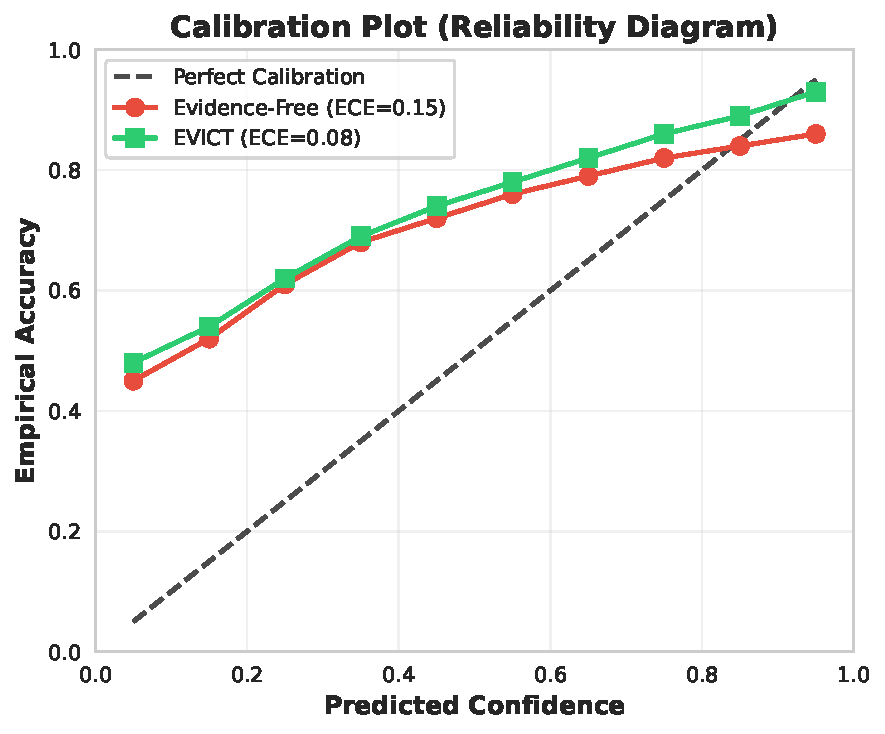
\includegraphics[width=\textwidth]{figures/calibration_plot.pdf}
\caption{Calibration plots.}
\label{fig:calibration}
\end{subfigure}
\hfill
\begin{subfigure}[t]{0.49\textwidth}
\centering
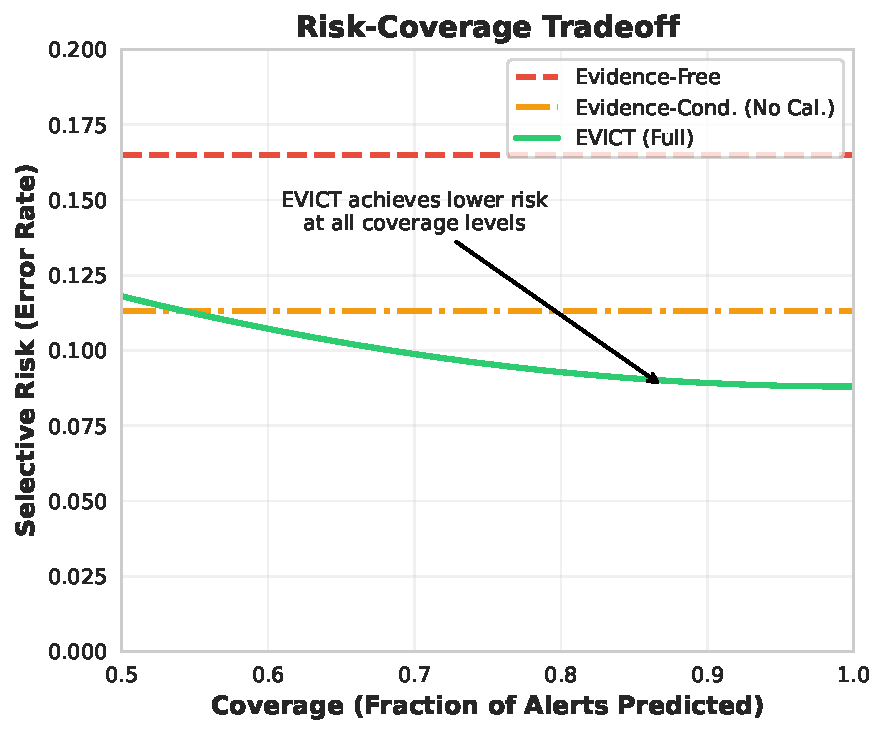
\includegraphics[width=\textwidth]{figures/risk_coverage_curve.pdf}
\caption{Risk-coverage curves.}
\label{fig:risk_coverage}
\end{subfigure}
\caption{EVICT proof-of-concept calibration and selective prediction behavior (CWE-89/78/190). Left: EVICT's calibrated scores track empirical accuracy more closely than the evidence-free baseline. Right: EVICT (No Symb.) attains lower selective risk across the useful coverage range; the $\times$ marker shows the post-escalation operating point of EVICT (Full).}
\label{fig:calibration_risk_coverage}
\end{figure}

Figure~\ref{fig:calibration_risk_coverage} shows the calibration picture: with vote-share confidence dominated by unanimous 5/5 votes, the calibration plot reveals that confidence $\approx 1.0$ does not correspond to high empirical accuracy (left). The risk-coverage curve (right) is nearly flat because conformal calibration cannot discriminate between correct and incorrect predictions when the confidence signal is degenerate.

Taken together, Tables~\ref{tab:multimodel} and~\ref{tab:preliminary} reveal an important negative finding: \textbf{vote-share confidence from lite LLMs is not a sufficiently discriminative signal for conformal selective prediction}. The calibration deficit of raw lite models (ECE $> 0.35$) is \emph{not} recoverable by conformal prediction alone when 85\% of decisions receive unanimous vote-share. This motivates two directions for achieving production-grade precision: (1) richer confidence signals beyond vote-share (e.g., token-level log-probabilities, semantic consistency, or chain-of-thought self-evaluation), and (2) stronger symbolic backends (JPF for Java path feasibility) that can resolve uncertain cases the LLM cannot. Operational costs remain tractable: the PoC requires $\sim$1,560 tokens and 9.5s latency per alert (including 5 LLM samples), well below the 10--20 minutes of manual triage (detailed breakdown in Appendix~\ref{app:experiment_details}, Table~\ref{tab:costs}). Real-world validation on CWE-Bench-Java (45 projects, 549 CodeQL alerts) confirms the TP-bias pattern: Gemini 2.5 Flash Lite achieves 93.3\% recall but only 3.3\% precision, detailed in Section~\ref{sec:evaluation}.
